\documentclass[a4paper,12pt]{report}
\addtolength{\oddsidemargin}{-1.cm}
\addtolength{\textwidth}{2cm}
\addtolength{\topmargin}{-2cm}
\addtolength{\textheight}{3.5cm}
\newcommand{\HRule}{\rule{\linewidth}{0.5mm}}
\makeindex


\usepackage[pdftex]{graphicx}
\usepackage{makeidx}
\usepackage{hyperref}
\hypersetup{
    colorlinks=true,
    linkcolor=blue,
    filecolor=magenta,      
    urlcolor=cyan,
}


% define the title
\author{Group6_a}
\title{ Assignment 1 Report}
\begin{document}
\setlength{\parskip}{6pt}

% generates the title
\begin{titlepage}

\begin{center}
% Upper part of the page       

\includegraphics[width=1\textwidth]{./up-logo.jpg}\\[0.4cm]    
\textsc{\LARGE Department of Computer Science}\\[1.5cm]
\textsc{\Large COS 301 - Software Engineering}\\[0.5cm]
% Title
\HRule \\[0.4cm]
{ \huge \bfseries COS 301 - Mini Project}\\[0.4cm]
\HRule \\[0.4cm]
% Author and supervisor
\begin{minipage}{0.4\textwidth}
\begin{flushleft} \large
\emph{Author:}\\
Hanrich {Potgieter}
\end{flushleft}
\end{minipage}
\begin{minipage}{0.4\textwidth}
\begin{flushright} \large
\emph{Student number:} \\
u12287343
\end{flushright}
\end{minipage}
\begin{minipage}{0.4\textwidth}
\begin{flushleft} \large
Chris {Cloete}
\end{flushleft}
\end{minipage}
\begin{minipage}{0.4\textwidth}
\begin{flushright} \large
\emph{} \\
u13029721
\end{flushright}
\end{minipage}
\begin{minipage}{0.4\textwidth}
\begin{flushleft} \large
Jason Richard {Evans}
\end{flushleft}
\end{minipage}
\begin{minipage}{0.4\textwidth}
\begin{flushright} \large
\emph{} \\
u13032608
\end{flushright}
\end{minipage}
\begin{minipage}{0.4\textwidth}
\begin{flushleft} \large
Kale-ab {Tessera}
\end{flushleft}
\end{minipage}
\begin{minipage}{0.4\textwidth}
\begin{flushright} \large
\emph{} \\
u13048423
\end{flushright}
\end{minipage}
\begin{minipage}{0.4\textwidth}
\begin{flushleft} \large
Lelethu {Zazaza}
\end{flushleft}
\end{minipage}
\begin{minipage}{0.4\textwidth}
\begin{flushright} \large
\emph{} \\
u13028023
\end{flushright}
\end{minipage}
\begin{minipage}{0.4\textwidth}
\begin{flushleft} \large
Goodness {Adegbenro}
\end{flushleft}
\end{minipage}
\begin{minipage}{0.4\textwidth}
\begin{flushright} \large
\emph{} \\
u13046412
\end{flushright}
\end{minipage}
\begin{minipage}{0.4\textwidth}
\begin{flushleft} \large
Herman Willem {Keuris}
\end{flushleft}
\end{minipage}
\begin{minipage}{0.4\textwidth}
\begin{flushright} \large
\emph{} \\
u13037618
\end{flushright}
\end{minipage}
\begin{minipage}{0.4\textwidth}
\begin{flushleft} \large
William {Seloma}
\end{flushleft}
\end{minipage}
\begin{minipage}{0.4\textwidth}
\begin{flushright} \large
\emph{} \\
u10155865
\end{flushright}
\end{minipage}
\vfill
% Bottom of the page
{\large \today}
\end{center}
\end{titlepage}
\footnotesize
<<<<<<< HEAD
%%
%%  University of Pretoria - Declaration of Originality
%%  Version: S4726/09 (amended 2010-07-23)
%%

\newpage

\thispagestyle{empty}
{
\renewcommand{\baselinestretch}{1}
\sffamily
\begin{center}
\textbf{\Large DECLARATION OF ORIGINALITY}
\end{center}
\begin{center}
\textbf{\large UNIVERSITY OF PRETORIA}
\end{center}

The University of Pretoria places great emphasis upon integrity and
ethical conduct in the preparation of all written work submitted for
academic evaluation.

While academic staff teach you about referencing techniques and how to
avoid plagiarism, you too have a responsibility in this regard. If you
are at any stage uncertain as to what is required, you should speak to
your lecturer before any written work is submitted.

You are guilty of plagiarism if you copy something from another
author's work (e.g. a book, an article or a website) without
acknowledging the source and pass it off as your own. In effect you
are stealing something that belongs to someone else. This is not only
the case when you copy work word-for-word (verbatim), but also when
you submit someone else's work in a slightly altered form (paraphrase)
or use a line of argument without acknowledging it. You are not
allowed to use work previously produced by another student. You are
also not allowed to let anybody copy your work with the intention of
passing if off as his/her work.

Students who commit plagiarism will not be given any credit for
plagiarised work. The matter may also be referred to the Disciplinary
Committee (Students) for a ruling. Plagiarism is regarded as a serious
contravention of the University's rules and can lead to expulsion from
the University.

The declaration which follows must accompany all written work
submitted while you are a student of the University of Pretoria. No
written work will be accepted unless the declaration has been
completed and attached.

\begin{center}
\begin{tabular}{ll}
                        &                             \\
 Full names of student: & \makebox[3.5in]{\hrulefill} \\ \\
 Student number:        & \makebox[3.5in]{\hrulefill} \\ \\
 Topic of work:         & \makebox[3.5in]{\hrulefill} \\ \\
\end{tabular}
\end{center}

\textbf{Declaration}
\begin{enumerate}
\item I understand what plagiarism is and am aware of the University's
  policy in this regard.
\item I declare that this assignment report is my own original work.
  Where other people's work has been used (either from a printed source,
  Internet or any other source), this has been properly acknowledged and
  referenced in accordance with departmental requirements.
\item I have not used work previously produced by another student or any
  other person to hand in as my own.
\item I have not allowed, and will not allow, anyone to copy my work with
  the intention of passing it off as his or her own work.
\end{enumerate}

\vspace*{1cm}

SIGNATURE: \makebox[3in]{\hrulefill} \quad DATE: \makebox[1.5in]{\hrulefill}
}

\newpage


=======
%%
%%  University of Pretoria - Declaration of Originality
%%  Version: S4726/09 (amended 2010-07-23)
%%

\newpage

\thispagestyle{empty}
{
\renewcommand{\baselinestretch}{1}
\sffamily
\begin{center}
\textbf{\Large DECLARATION OF ORIGINALITY}
\end{center}
\begin{center}
\textbf{\large UNIVERSITY OF PRETORIA}
\end{center}

The University of Pretoria places great emphasis upon integrity and
ethical conduct in the preparation of all written work submitted for
academic evaluation.

While academic staff teach you about referencing techniques and how to
avoid plagiarism, you too have a responsibility in this regard. If you
are at any stage uncertain as to what is required, you should speak to
your lecturer before any written work is submitted.

You are guilty of plagiarism if you copy something from another
author's work (e.g. a book, an article or a website) without
acknowledging the source and pass it off as your own. In effect you
are stealing something that belongs to someone else. This is not only
the case when you copy work word-for-word (verbatim), but also when
you submit someone else's work in a slightly altered form (paraphrase)
or use a line of argument without acknowledging it. You are not
allowed to use work previously produced by another student. You are
also not allowed to let anybody copy your work with the intention of
passing if off as his/her work.

Students who commit plagiarism will not be given any credit for
plagiarised work. The matter may also be referred to the Disciplinary
Committee (Students) for a ruling. Plagiarism is regarded as a serious
contravention of the University's rules and can lead to expulsion from
the University.

The declaration which follows must accompany all written work
submitted while you are a student of the University of Pretoria. No
written work will be accepted unless the declaration has been
completed and attached.

\begin{center}
\begin{tabular}{ll}
                        &                             \\
 Full names of students: & \makebox[3.5in]{\hrulefill} \\ \\
 Student numbers:        & \makebox[3.5in]{\hrulefill} \\ \\
 Topic of work:         & \makebox[3.5in]{\hrulefill} \\ \\
\end{tabular}
\end{center}

\textbf{Declaration}
\begin{enumerate}
\item I understand what plagiarism is and am aware of the University's
  policy in this regard.
\item I declare that this assignment report is my own original work.
  Where other people's work has been used (either from a printed source,
  Internet or any other source), this has been properly acknowledged and
  referenced in accordance with departmental requirements.
\item I have not used work previously produced by another student or any
  other person to hand in as my own.
\item I have not allowed, and will not allow, anyone to copy my work with
  the intention of passing it off as his or her own work.
\end{enumerate}

\vspace*{1cm}

SIGNATURES: \makebox[3in]{\hrulefill} \quad DATE: \makebox[1.5in]{\hrulefill}
}

\newpage


>>>>>>> c9c34b47029f66b93ead74067c518a6171377c84

\normalsize

\renewcommand{\thesection}{\arabic{section}}
\newpage
\begin{center}
\textsc{\LARGE Software Requirements Specification and Technology Neutral Process Design}\\[1.5cm]
\textsc{\Large Buzz Space Discussions/Mini Project}\\[0.5cm]
Version: Version 0.2 Alpha 
For further references see \href{ https://github.com/DieBaber/COS301-GROUP6-A.git}{gitHub}.
\today
\end{center}
\tableofcontents{}
For further references see \href{https://github.com/DieBaber/COS301-GROUP6-A.git}{gitHub} or got to the link https://github.com/DieBaber/COS301-GROUP6-A.git
\section{Functional requirements}
	\begin{center}
  	 	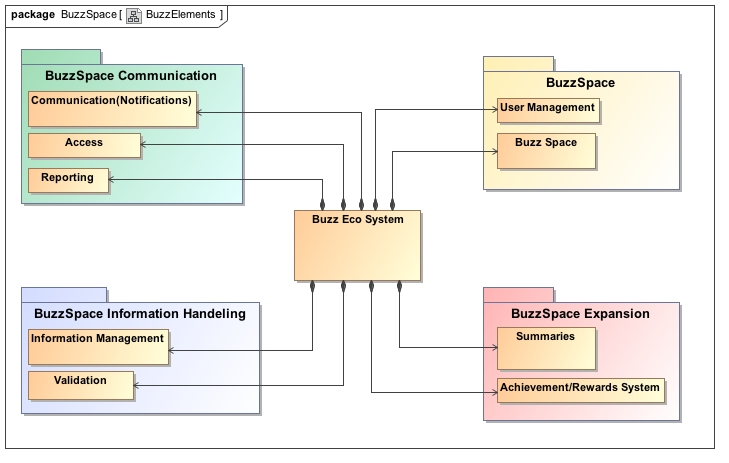
\includegraphics[width=1\textwidth] {../Hanrich/BuzzElements.jpg}\\[0.4cm]    
	\end{center}
\subsection{Introduction}
We use this document to give a high level overview of the buzz  discussion board. We have identified the various components. Our purpose is to create a dynamic and scalable solution. We also want to include an achievement system that rewards users for using the discussion board. This document will inform you on how we will achieve a system that is both scalable and pluggable. We have identified the use cases of the various components of the discussion board.
\newpage
\subsection{Use case prioritiation}
\textbf{Critical} 
\begin{itemize}
  \item BuzzSpace
  \item CRUD posts(Creating,Reading; Updating; Deleting).
  \item System Access
  \item Information Management
  \item User restriction
  \item Automatic update of Status
  \end{itemize}
\textbf{Important} 
\begin{itemize}
  \item User Management
  \item Communication(Notifications)
  \item Reporting
\end{itemize}
\textbf{Nice-To-Have} 
\begin{itemize}
  \item Achievement/Rewards System
  \item Reporting
  \item Summaries
\end{itemize}
\subsection{Use case/Service contracts}
\begin{center}
  \begin{tabular}{ p{3cm} | p{4cm} | p{4cm} | p{4cm} }
    \hline
    Use Case & Pre Condition & Post Condition & Description \\ \hline \hline
    BuzzSpace & There must be a valid user & User must still exist & \\ \hline
    Information Management &  &  &\\ \hline
    Communication&  &  & \\ \hline
    Summaries &  &  & \\ \hline
    Achievement Rewards System & A user's level requires Achievements to be allocated and/or rewards to be awarded & Achievements are allocated and/or rewards are awarded & \\ \hline
    Summaries  & &  & \\ \hline
    Access &  &  & \\ \hline
    Summaries &  &  & \\ \hline
    Validation & Post is palgiarised and/or does not follow netiquette & Post is valid against rules  & \\ \hline
    User Management &  &  & \\ \hline
    Reporting & Data must be available to report on. & Data must not be corrupt. & This use case generate report for all actors\\ \hline
    Automatic update of the user status & User is logged in , Nothing is posted and old status remains. & User posted and status updated,  or User logged out and not updated status old status remains & User logs in and updates his or her status and status is updated \\ \hline
    \hline
  \end{tabular}
\end{center}
\subsection{Required functionality}
\begin{itemize}
\newpage
	\item \textbf{BuzzSpace}
	% We need to add the correct pictures here. We must also give a description of the elements.
		\begin{center}
  	 	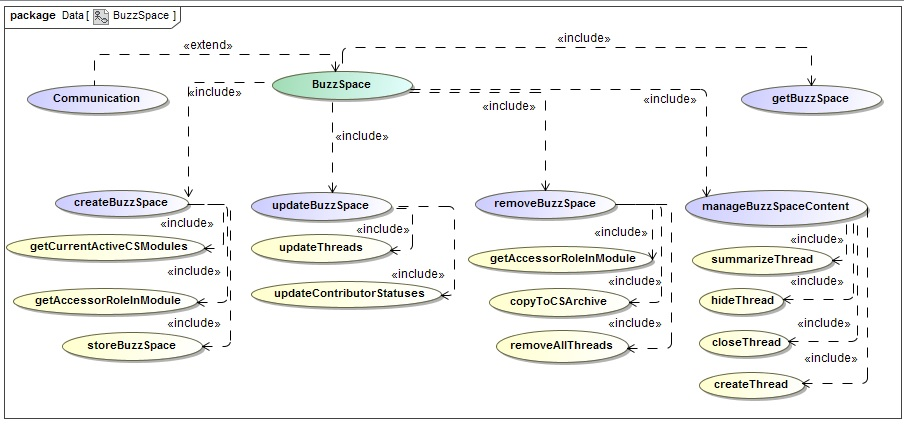
\includegraphics[width=1\textwidth] {../Lelethu/UseCase_BuzzSpace.jpg}\\[0.4cm]    
		\end{center}
\newpage
\item \textbf{Validation}. This module will be used to make sure that post follow certain rules and help generate certain reports regarding these rules.
		\begin{center}
  	 	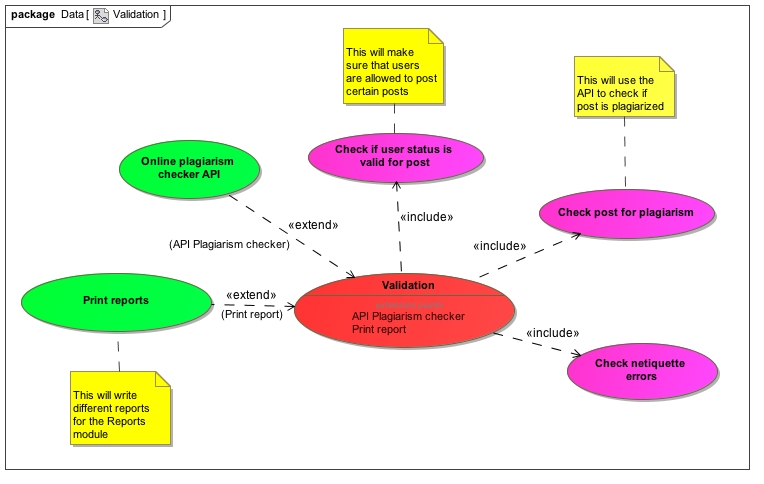
\includegraphics[width=1\textwidth] {../Chris/Validation.jpg}\\[0.4cm]    
		\end{center}
\newpage
	\item  \textbf{Information Management}
		\begin{center}
  	 	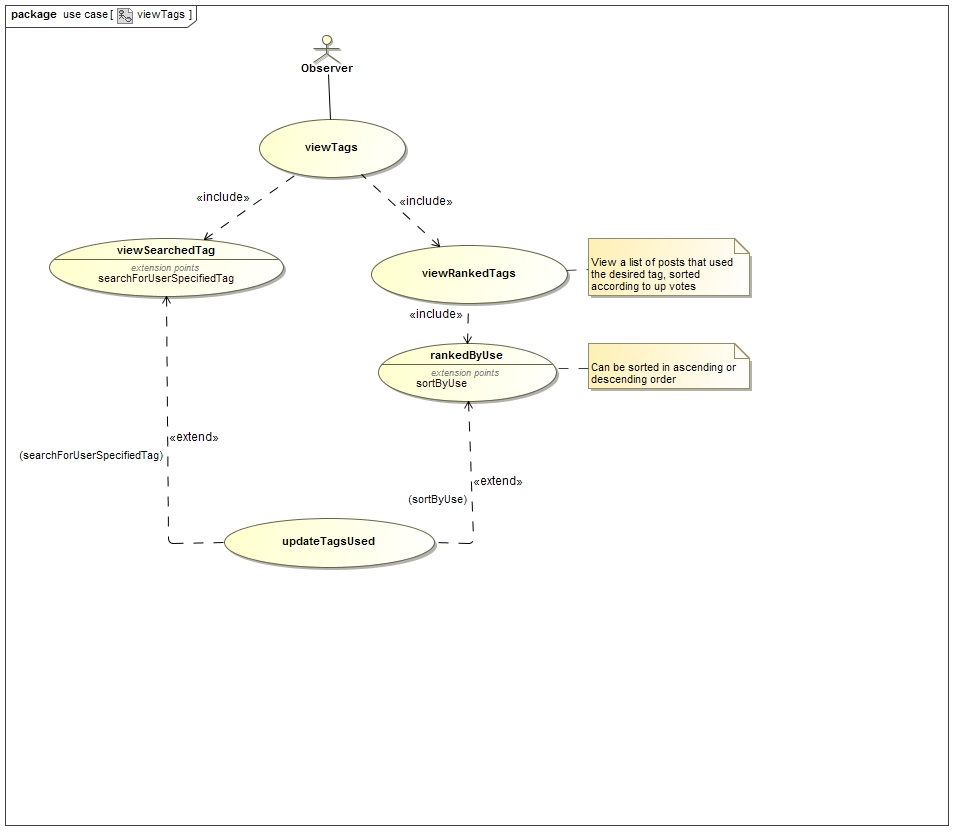
\includegraphics[width=1\textwidth] {../Herman/viewTags.jpg}\\[0.4cm]    
		\end{center}
	\item \textbf{Reporting}. We will use the reporting module to generate quite a few reports regarding the Buzz Space system. It will be a key player in adding value to lecturers and students. Each student can easily general a report regarding their own contributions towards a Buzz Space. Lecturers will be able to grade student performance and see how much plagiarism has occurred. The system administrators will be able to check for system bugs and see error logs. 
		\begin{center}
  	 	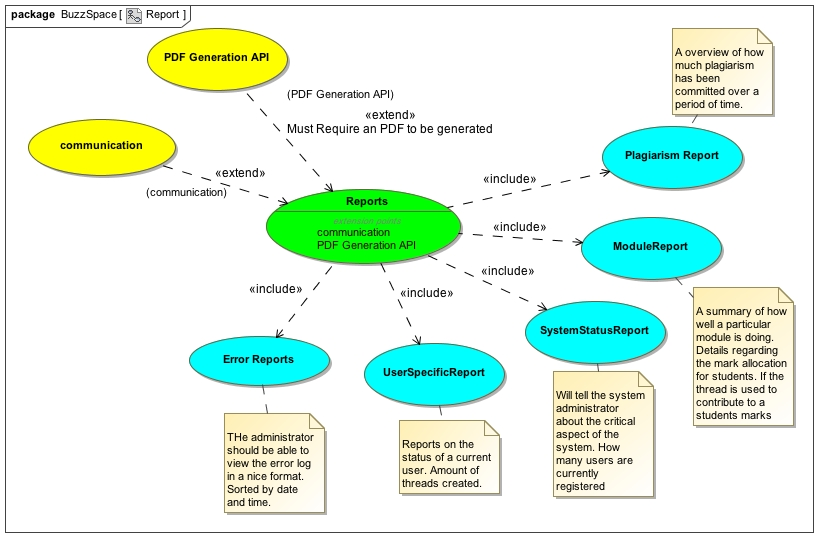
\includegraphics[width=1\textwidth] {../Hanrich/Report.jpg}\\[0.4cm]    
		\end{center}
\end{itemize}
\subsection{Process specification}
We want to show various important process specification of our recommendation.
\begin{itemize}
	\item CreateBuzzSpace
		\begin{center}
  	 	\includegraphics[width=1\textwidth] {../Functional_Requirements_Diagrams/ActivityDiagrams/ActivityDIagram_UpdateBuzzSpace.jpg}\\[0.4cm]    
		\end{center}
	\item Validation
		\begin{center}
  	 	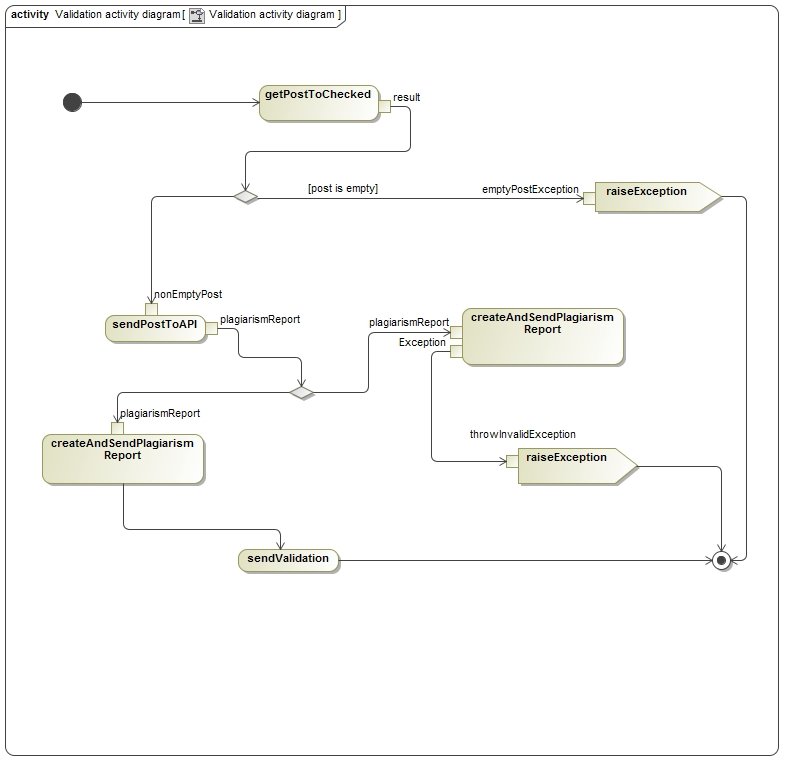
\includegraphics[width=1\textwidth] {../Chris/Validationactivitydiagram.jpg}\\[0.4cm]    
		\end{center}
\end{itemize}
\subsection{Domain Model}
\index{Vision}
\newpage


\bibliography{myrefs}{} 
\bibliographystyle{ieeetr}
\end{document}
